\documentclass[11pt,a4paper]{article}
\usepackage[utf8]{inputenc}
\usepackage{amsmath}
\usepackage{amsfonts}
\usepackage{amssymb}
\usepackage[backend=biber,style=numeric,url=true]{biblatex} % für Quellenangaben und Bibliotheken
\usepackage[]{hyperref} % für hyperlinks
\author{Moritz Ruge}

% Paket für die Baumdiagramdarstellung
\usepackage{tikz}
\usetikzlibrary{trees}

\hypersetup{
    colorlinks=true,
    linkcolor=blue,
    filecolor=magenta,      
    urlcolor=cyan,
    pdftitle={Overleaf Example},
    pdfpagemode=FullScreen,
    }


\begin{document}

% Aufgabe 1 Binäre Suchbäume)


			% Aufgabe 1 a

\begin{itemize}
\item Einfügen des gesamten Schlüssels:
\end{itemize}

% Alle schlüssel eingefügt
\begin{tikzpicture}[scale=0.4]

\node {A}
	child[missing]
	child{ node{L}
	  child{ node{G}
	    child{ node{D}}
	    child[missing]}
	  child{ node{O}
	    child[missing]
	    child{ node{T}
	      child{node{S}}
	      child{node{X}
	        child[missing]
	        child{node{Y}
	          child[missing]
	          child{node{Z}}}}}}};
\end{tikzpicture}

% Löschen von Schlüssel Z
\begin{itemize}
\item Löschen von Schlüssel $Z$
\end{itemize}

\begin{tikzpicture}[scale=0.4]

\node {A}
	child[missing]
	child{ node{L}
	  child{ node{G}
	    child{ node{D}}
	    child[missing]}
	  child{ node{O}
	    child[missing]
	    child{ node{T}
	      child{node{S}}
	      child{node{X}
	        child[missing]
	        child{node{Y}}}}}};
\end{tikzpicture}

% Löschen von Schlüssel A
\begin{itemize}
\item Löschen von Schlüssel $A$
\end{itemize}

\begin{tikzpicture}[scale=0.4]

\node {L}
	  child{ node{G}
	    child{ node{D}}
	    child[missing]}
	  child{ node{O}
	    child[missing]
	    child{ node{T}
	      child{node{S}}
	      child{node{X}
	        child[missing]
	        child{node{Y}}}}};
\end{tikzpicture}

% Löschen von Schlüssel L
\begin{itemize}
\item Löschen von Schlüssel $L$
\end{itemize}

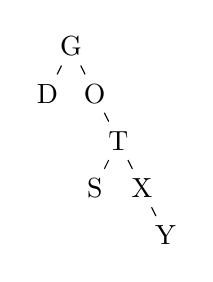
\begin{tikzpicture}[scale=0.4]

\node {G}
	    child{ node{D}
	    child[missing]}
	  child{ node{O}
	    child[missing]
	    child{ node{T}
	      child{node{S}}
	      child{node{X}
	        child[missing]
	        child{node{Y}}}}};
\end{tikzpicture}
\end{document}